\documentclass{article}
\usepackage[utf8]{inputenc}
\usepackage{graphicx}
\usepackage{here}

\title{Notes de cours\\TC4 : Algorithmes d'inférence et matricielles à grande échelle}
\author{Adrien Pavao}
\date{Septembre 2017}

\begin{document}

\maketitle

\tableofcontents

\section{Définitions et formules}

\subsection{Notions générales}

\begin{itemize}
\item \textbf{Variable aléatoire :} Une fonction définie depuis l'ensemble des résultats possibles d'une expérience aléatoire, dont on doit pouvoir déterminer la probabilité qu'elle prenne une valeur donnée ou un ensemble donné de valeurs. 

Cette variable peut être discrète ou continue.

Dans le cas d'une variable discrète, la fonction masse est la fonction qui donne la probabilité d'un résultat élémentaire d'une expérience.

Dans le cas d'une variable continue, la distribution de la masse de probabilité est caracterisée par la densité de probabilité f(x) : 

\[ P(a < X \leq b)  = \displaystyle \int_{a}^{b} f(x) \, \mathrm{d}x \]

\item \textbf{Réalisations :} Les réalisations d'une variable aléatoire sont les résultats des valeurs choisies au hasard en fonction de la loi de probabilité de la variable. On les appelle également les variations aléatoires.

\item \textbf{Distribution (loi de probabilité) :} Le concept de loi de probabilité se formalise mathématiquement à l'aide de la théorie de la mesure : une loi de probabilité est une mesure, souvent vue comme la loi décrivant le comportement d'une variable aléatoire, discrète ou continue. Une mesure est une loi de probabilité si sa masse totale vaut 1. L'étude d'une variable aléatoire suivant une loi de probabilité discrète fait apparaître des calculs de sommes et de séries, alors que si sa loi est absolument continue, l'étude de la variable aléatoire fait apparaître des calculs d'intégrales.

\item \textbf{Inférence :} Trouver la valeur des v.a. à partir d'autres qui sont connues.

\item \textbf{Vraisemblance :} $P(D; \Theta)$ avec D les données d'estimation et $\Theta$ l'ensemble des paramètres.

\item \textbf{Estimation :} Retrouver les paramètres d'une distribution à partir de l'observation d'un ensemble de réalisations de celle-ci. Il s'agit du maximum de vraisemblance.

\item \textbf{Sampling :} Générer des données.

\end{itemize}

\subsection{Différentes probabilités liées}

\begin{itemize}

\item \textbf{Probabilité jointe :} Probabilité d'une configuration donnée. On note $P(X, Y)$. Il s'agit de la probabilité de la réalisation de l'évenement X \textbf{et} de l'évenement Y.

\item \textbf{Probabilité conditionnelle :} La probabilité de X sachant Y se note $P(X|Y)$. Pour faire simple, on fixe la variable connue.

\[ P(X|Y) = \frac{P(X, Y)}{P(Y)} \]
 
\item \textbf{Probabilité marginale :} On vire une variable en la sommant. A partir de $P(X = x, Y = y)$, on peut obtenir :

\[ P(X = x) = \sum_{y} P(X = x, Y = y) \]

\end{itemize}

La probabilité jointe inclus les deux autres. On peut retrouver la distribution jointe à partir de la distribution conditionnelle et
marginale.


\subsection{Moyenne, variance, covariance et corrélation}

Soit $x_1$, $x_2$, ..., $x_n$ un ensemble de valeurs générées par une distribution de probabilité inconnue. On peut caractériser cette distribution par : 

\begin{itemize}
\item La \textbf{moyenne}, qui caractérise le \textbf{centre} de la distribution.

\[ \bar{x} = \frac{1}{n} \sum_{i=1}^{n} x_i \]

\item La \textbf{variance}, qui mesure la \textbf{dispersion} de la distribution.


\[ \frac{1}{n} \sum_{i=1}^{n} (x_i - \bar{x})^{2} \]

\[ var(x) = \frac{1}{N} \sum_{n=1}^{N} (x_n - \bar{x})^2 \]


\item L'\textbf{écart-type}, qui est la racine carrée de la variance.

$\sigma = \sqrt{var(x)}$

\item La symétrie ou l'asymétrie (skewness).

\begin{figure}[H]
   \caption{Schéma représentatif de la skewness}
    \begin{center} 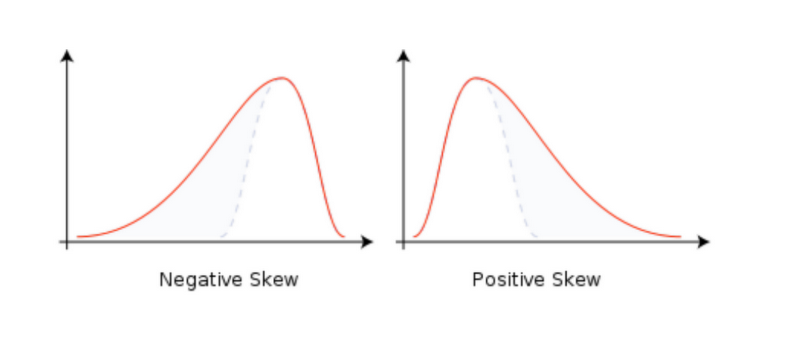
\includegraphics[scale=0.4]{skewness.png} \end{center}
\end{figure}


\item La covariance, le lien entre les variations de deux variables.

\[ cov(x, y) = \frac{1}{N} \sum_{n=1}^{N} (x_n - \bar{x}) (y_n - \bar{y}) \]

\item La corrélation, une covariance normalisée. Elle quantifie la qualité de l'approximation linéaire de x par y, et reciproquement.

\[ cor(x, y) = \frac{cov(x, y)}{var(x) var(y)} = \frac{cov(x, y)}{cov(x, x) cov(y, y)} \]


\end{itemize}


Pour les V.A. multidimensionnelles, on a la \textbf{matrice de covariance}.

\subsection{Indépendance statistique}

\begin{itemize}

\item \textbf{Variables indépendantes :} Deux variables sont indépendantes si et seulement si :

\[ P(X = x, Y = y) = P(X = x) \times P(Y = y) \]

\item \textbf{Variables conditionnellement indépendantes :} Deux variables sont conditionnellement indépendantes si et seulement si :

\[ P(X = x, Y = y | Z = z) = P(X = x | Z = z) \times P(Y = y | Z = z) \]

\item \textbf{Indépendantes et identiquement distribuées (i.i.d) :} Ce dit de deux variables indépendantes suivant la même loi de probabilité. Il sera souvent nécessaire de poser cette hypothèse. On en déduit : $P(X_{1, N} ) = \prod_{1}^{N} P(X_i)$

\end{itemize}

\subsection{Théorème de Bayes}

\[ P(Y = y_j | X = x_i) = \frac{P(X = x_i | Y = y_j) P(Y = y_j)}{\sum_{y_j \in A_y} P(X = x_i | Y = y_j) P(Y = y_j)} \]

\[ P(Y = y_j | X = x_j) = \frac{P(X = x_i | Y = y_j) P(Y = y_j)}{P(X = x_i)} \]

\subsection{Lois de probabilités courantes}

\begin{tabular}{|l|l|c|l|}
  \hline
  Loi & Type de la V.A. & Formule & Paramètres \\
  \hline
  Bernouilli & Binaire & $p^x(1-p)^{1-x}$ & p \\
  Binomiale & Discrète & $C^{k}_{n} \times p^k \times (1-p)^{n-k}$ & n, p \\
  Poisson &Discrète & $\frac{\lambda^k}{k!} \times e^{- \lambda} $ & $\lambda$ \\
  Normale dimension 1 & Continue & $\frac{1}{\sigma \sqrt{2 \pi}} \times e^{\frac{-1}{2}(\frac{x - \mu}{\sigma})^2} $ & $\mu$, $\sigma$ \\
  Normale dimension d & Continue& $\frac{1}{(2 \pi)^{\frac{d}{2}} ||\Sigma||^{\frac{1}{2}}} \times e^{- \frac{1}{2} (x - \mu)^t \Sigma^{-1} (x - \mu)}$ & $\mu$, $\Sigma$ \\ 
  \hline
\end{tabular}


\section{Classification bayésienne}

Note : A completer.

Soit les points suivantes:

\begin{itemize}
\item Variable aléatoire X, une observation à classer.
\item Variable aléatoire Y, désignant la classe à affecter à X.
\item Décision $\alpha_i$, affectation de x à la classe $y = i$.
\item Fonction de perte $\lambda(\alpha_i | j)$, décision $\alpha_i$ alors que la classe correcte était j.
\end{itemize}

Sur l'observation x, l'espérance du risque de décider $\alpha_i$ est : 

\[ R(\alpha_i | x) = \sum_{j = 1}^{k} \lambda(\alpha_i | j) P(Y = j | x) \]

\section{Modèles de Markov Cachés (H.M.M.)}

\subsection{Introduction et exemple}

\subsubsection{Robotique} 

Un robot doit détecter votre état. 
\begin{itemize}

\item 1 V.A. y : état de la personne, $A_y = {t^0, h^1}$ \\
      La variable à inférer.

\item Le robot reçoit une observation $X(1 V.A.)$, $A_x = {dormir, pleurer, tv, manger, tw}$\\
      Le but est d'estimer $P(Y = y | X = x)$

\end{itemize}

\subsubsection{Un modèle simple} 

Classification Bayésienne. On doit estimer $P(X = x, Y = y) = P(X = x | Y = y) P(Y = y)$

$P(X = x | Y = y)$, l'observation qu'on peut représenter par un tableau : 
\begin{tabular}{|l|l|l|l|l|l|}
  \hline
  - & d & p & t & m & t \\
  \hline
  0 & 0, 1 & 0, 2 & 0, 5 & 0, 1 & 0, 1 \\
  1 & 0, 2 & 0, 1 & 0, 2 & 0, 2 & 0, 3 \\
  \hline
\end{tabular}

La somme de chaque ligne doit être égal à 1. 

$P(Y = y)$, l'a priori en Y.

Etat caché Y $\rightarrow$ Observation X.

\subsubsection{Un modèle dynamique} 

Modéliser l'évolution au cours du temps (discret). On prend en compte les transitions et dépendances entre états.

\textbf{Modification.} 
\begin{itemize}
\item $Y_t$ : l'état est situé dans le temps.
\item $X_t$ : l'état est situé dans le temps.
\end{itemize}

Schema mytho.

Impact de cette hypothèse sur les paramètres : 
\begin{itemize}
\item Distribution sur les observations : $P(X_t | Y_t)$
\item Distribution sur les transitions : $P(Y_t | Y_{t - 1})$
      \begin{tabular}{|l|l|l|}
        \hline
        $Y_t, Y_{t-1}$ & 0 & 1 \\
        \hline
        0 & 0,99 & 0,1 \\
        1 & 0,01 & 0,9 \\
        \hline
      \end{tabular}

Schema automate.

\item Distribution (de l'état) initiale : $P(Y_1)$
\end{itemize}

\subsection{Définition d'un H.M.M}

Un modèle H.M.M. (Hidden Markov Model) : 
\begin{itemize}
\item L'ensemble des états S (N états possibles)
\item L'ensemble des observations : $A_x$
\item A chaque instant t (temps discret) :
  \begin{itemize}
  \item Changer d'état d'après une distribution de transition $Y_{t-1 \rightarrow Y_t}$
  \item Engendrer une observation : $Y_t \rightarrow X_t$
  \end{itemize}
\item A partir d'un état initiale $Y_1$ 
\end{itemize}

Les donnée associées : ((séquence d'obervations), (séquence d'états))
\begin{itemize}
\item 2 séquences de même longueur
\item On observe un modèle de Markov sur T instants. $(X_{1:T}, Y_{1:T})$ \\ $ X_{1:T} = (X_1, X_2, ..., X_T) $
\end{itemize}

\subsubsection{Hypothèses Markoviennes}

Un H.M.M. définit une distribution sur $P(X_{1:T}, Y_{1:T}) = P(X_1, ..., X_T, Y_1, ..., Y_T)$

\[ P(X_{1:T}, Y_{1:T}) = P(X_{1:T} | Y_{1:T}) P(Y_{1:T})  \]

\begin{itemize}
\item Observations : $P(X_{1:T} | Y_{1:T})$
\item Transitions : $P(Y_{1:T})$
\end{itemize}

Schema mytho. \\

\textbf{Hypothèse de Markov 1 :} L'état $Y_t$ ne dépend que de l'état précédent. \\

Formellement, on a :

\[ P(Y_{1:T}) = P(Y_1) \times P(Y_2 | Y_1) \times P(Y_3 | Y_1, Y_2) \times ... \times P(Y_T | Y_1, Y_2, ..., Y_{T-1}) \]

Mais l'hypothèse de Markov, bien que souvent fausse, permet de simplifier grandement ce calcul de probabilité. Ainsi, on a :

\[ P(Y_{1:T}) = P(Y_1) \times P(Y_2 | Y_1) \times ... \times P(Y_T | Y_{T-1}) \]

\textbf{Hypothèse de Markov 2 :} L'observation $X_t$ ne dépend que de $Y_t$. \\

Normalement, on a :

\[ P(X_{1:T} | Y_{1:T}) = P(X_1 | Y_{1:T}) \times P(X_2 | X_1, Y_{1:T}) \times ... \times P(X_T | X_{1:T-1}, Y_{1:T}) \]

En appliquant l'hypothèse, souvent fausse également, on obtient :

\[ P = \Pi_{t = 1}^{T} P(X_t | Y_t)  \]

\subsubsection{Stationarité}

$ \forall t$ : $P(X_t | Y_t)$ et $P(Y_t | Y_{t - 1})$ sont inchangées.

\subsubsection{Les paramètres}
Les paramètres sur un modèle de Markov sont : 

\begin{itemize}
\item Une distribution initiale : $|S|$
\item Une distribution de transitions : $|S|^2$
\item Une distribution d'observations : $|A_x| \times |S|$
\end{itemize}

On les représente par des matrices. On nomme la matrice de transitions A et la matrice d'observations B.

\subsection{Applications}

\begin{itemize}
\item Reconnaissance de la parole, Tracking vidéo, Reconnaissance optique de caractères, finance et prédiction de marché.
\item P.O.S. Tagging (Part of Speech) (NLP)
\item Apprentissage supervisé : $D_S = ((X_{1:T}), (Y_{1:T}))$. Un H.M.M. est un modèle génératif.
\item Apprentissage non supervisé, car c'est un modèle génératif. On induit les clusters (classes). $D_N = (X_{1:T})$
\item Apprentissage semi-supervisé, grâce aux deux précédents : $D = D_S + D_N$.
\end{itemize}

\subsection{Inférence}

La question d'inférence : $ P(Y_i | X_{1:i}$ ?

Si on reprend l'exemple du robot : $P(Y_3 = t | X_{1:4} = (r, tw, P))$

\subsubsection{Enumération}

$$ P(Y_3 | X_{1:3}) = \sum_{y y} P(Y_1 = y1, Y_2 = y_2, Y_3 = y_3 | X_1:3) $$
$$ P(Y_3 | X_{1:3}) = \frac{P(X_{1:3}, Y_{1:3})}{P(X_{1:3})} $$

\subsubsection{Algorithme Forward}

$$ P(Y_{1:i} | X_{1:k} = \frac{\alpha(i, k)}{\sum_{j \ in S} \alpha(j, k)} $$
\\
Le dénominateur est la normalisation à 1.
\\
On utilisation pour la représentation une matrice. Chaque ligne représente un état, et chaque colonne un instant dans le temps.

\textbf{Calcul de $\alpha(i, k)$ :} Arriver à l'instant k dans l'état i.
$$ \alpha(i, k) = P(Y_{k:i}, X_{1:k}) $$
$$ \alpha(i, k) = P(X_1, X_2, ..., X_k, Y_k) $$
$$ \alpha(i, k) = P(X_k | Y_k, X_{1:k-1}) \times P(Y_k, X_{1:k-1})$$

\textbf{Calcul de $P(Y_k, X_{1:k-1})$ :}

$$ P(Y_k, X_{1:k-1}) = \sum_j P(Y_k, Y_{k-1:j}, X_{1:k-1}) $$
$$ [...] $$
$$ P(Y_k, X_{1:k-1}) = \sum_j \alpha(i ,j) \times \alpha(j, k-1) $$

\textbf{Conclusion :}

$$ \alpha(i, k) = b(x_k, i) \times \sum_{j \in S} [\alpha(i, j) \times \alpha(j, k-1)] $$

%% SCHEMA MYTHO 

L'\textbf{algorithme forward} consiste à calculer $\alpha(i, k)$. En voici les étapes : 
\begin{enumerate}
\item Création d'une matrice $M$ de taille $(|S|, k)$.
\item Initialiser la première colonne : $\alpha(i, 1) = \pi(i) \times b(x_1, i) $.
\item Pour $k' = 2$ à $k$ : Remplir la colonne $k'$ : $\alpha(i, k')$
\item Utilisation des $\alpha$.
    \begin{enumerate}
    \item \textbf{Prédiction} : $P(Y_{k:i} | X_{1:k}) = \frac{\alpha(i, k)}{\sum_j \alpha(j, k)}$
    \item \textbf{Evidence/Normalisation} : $P(X_{1:k}) = \sum_j \alpha(j, k)$
    \end{enumerate}
\item \textbf{Viterbi} : \\
Question : $y_{1:k}$ qui maximise $P(Y_{1:k} | X_{1:k})$, \\
Définir $\delta(i, k)$ la probabilité du  meilleur chemin permettant d'arriver à l'instant \textbf{k'} dans l'état \textbf{i}.
$$ \delta(i, k) = b(x_k, i) \times max_{j \in S} [ \alpha(i, j) \delta(j, k-1) ] $$
$$ \psi(i, k) = b(x_k, i) \times argmax [ \alpha(i, j) \delta(j, k-1) ] $$
\end{enumerate}

\subsubsection{Algorithme Backward}

A l'instant t, le modèle est dans l'état $Y_t = i$

\[ P(X_{t+1 : T} | Y_t = i) = \beta(i, t) \]

\[ \beta(i, t) = \sum_j \beta(j, t+1) a(j, i) b(x_{t+1}, j) \]

L'objectif est maintenant de calculer la matrice des '$\beta$' $(|S|, T)$ :
\begin{itemize}
\item On initialise : $\beta(i, T) = 1$
\item Récurrence de droite à gauche pour $t = (T-1):1$. On remarque que cela se fait de droite à gauche dans le cas de l'algorithme Backward.
\end{itemize}
Application : 
$$ P(X_{1:T}) = \sum_j \beta(j, 1) \pi(j) b(x_1, j) $$

\subsection{Forward - Backward}

\subsubsection{Décodage 'a posteriori' ou 'par position'}

L'objectif est d'inférer pour : $$X_{1:T} : Y_{1:T}$$ 

Pour chaque instant t : $$ y_t^* = argmax_{y_t} P(Y_t = g_t | X_{1:T}) $$

On cherche donc : $$P(Y_t = i | X_{1:T}) \propto P(Y_t = i, X_{1:T}) $$

$$ P(Y_t = i | X_{1:T}) \propto P(Y_t = i | X_{t+1:T}) \times P(X_{t+1:T} | Y_{t=i}, X_{1:T}) $$

On simplifie et on obtient : $$ P(Y_t = i | X_{1:T}) = \frac{\alpha(i, t) \beta(i, t)}{\sum_j \alpha(j, t) \beta(j, t)} $$

Remarque : $$ P(X_{1:T}) = \sum_j \alpha(j, t) \beta(j, t), \forall t $$

\subsubsection{Apprentissage non-supervisé}

\begin{itemize}
\item On doit fixer un nombre d'états.
\item Adapter E.M. pour les H.M.M : Baum-Welah.
\end{itemize}

$$ D = (X_{1:T}) $$ plutôt que $$ D_{sup} = (X_{1:T}, Y_{1:T}) $$

Des variables cachées $ Z \rightarrow P(Z | X) $ 
\\
\textbf{E.M.}
\begin{enumerate}
\item Etape E : Calcul les pseudo-affectations
$ P(Z | X)$ / à $\Theta$ fixé.
\item Etape M : re-estimation des $\Theta$ à partir des pseudos-affectations
\end{enumerate}

\textbf{Distribution de l'état initial}
\\
E : Pour chaque état possible : 
$$ P(Y_1 = i | X_{1:T}) = \frac{\alpha(i, 1) \beta(i, 1)}{\sum_j \alpha(j, 1) \beta(j, 1)} $$

\textbf{Distribution d'observation}
\\
Pour une séquence $X_{1:T}$, collecter $c(k, i)$ = nombre de fois où l'observation $x_t = k$ est engendrée par l'état i.

$$ \forall t : c(k, i)_t = P(Y_t = i | X_{1:T}) $$

\textbf{Exemple : } Une séquence 'the', 'cat', 'is', 'running' correspond à une séquence $x_1$, $x_2$, $x_3$, $x_4$.

$|S|$ = 
\begin{tabular}{|c|c|c|c|}
\hline
$x_1$ & $x_2$ & $x_3$ & $x_4$ \\
\hline
- & - & - & - \\
- & - & - & - \\
- & - & $\frac{\alpha(i, t) \beta(i, t)}{\sum_j \alpha(j, t) \beta(j, t)}$ & - \\ 
\hline
\end{tabular}

\begin{itemize}
\item Forward $\rightarrow \alpha$
\item Backward $\rightarrow \beta$
\item Combinaison + normalisation par colonne.
\end{itemize}

\textbf{Distribution des transitions}
\\
On aimerait $c(i, j)$
$$ c(i, j) \rightarrow P(Y_t = i, Y_{t-1} = j | X_{1:T}), \forall t > 1 $$
$$ P(Y_{t=i}, Y_{t-1=j} | X_{1:T}) \propto \alpha(j, t-1) \beta(i, t) a(i, j) b(x_t, i) $$

\subsubsection{Remarques}
\begin{enumerate}
\item E.M. dépend de l'état initial.
\item 'Etat initial'. On peut supprimer la notion d'état initial. On peut par exemple supposer un état "o", tanani...
\end{enumerate}

\end{document}


